\chapter{Background}

\section{Natural Language Processing}

Natural Language Processing (NLP) is a field of computer science and artificial intelligence that focuses on the interaction between computers and human language. It involves using techniques like machine learning and computational linguistics to help computers understand, interpret, and generate human language.

The previous example itself was an example of the applications of NLP, being an answer to a prompt given to ChatGPT \cite{ChatGPT}, a chatbot built on the 175 billion parameter GPT-3 model developed by OpenAI \cite{gpt_3}. It exemplifies how NLP empowers language models like ChatGPT to comprehend user queries, provide accurate responses, and maintain contextual awareness by recalling past conversations. By leveraging advanced machine learning techniques, ChatGPT exhibits the ability to understand and respond to prompts while retaining knowledge from ongoing interactions.

GPT-3, like other NLP models designed for interactive tasks, undergoes pre-training on an extensive corpus of conversational data. Furthermore, it can be fine-tuned for specific applications such as question answering, conversation generation, and text summarization. With its capacity to comprehend and generate natural language inputs, GPT-3, and other similar large language models, becomes a powerful tool for constructing chatbots and various conversational systems.

In addition to chatbots, NLP finds utility in text classification tasks. In this project, we focus on sentiment analysis for toxicity detection, a method in which an NLP model can be trained on a substantial dataset comprising of both hateful and benign messages, enabling it to learn patterns and characteristics indicative of hateful language.

\section{Recurrent Neural Networks}

\begin{figure}[H]
    \centering
    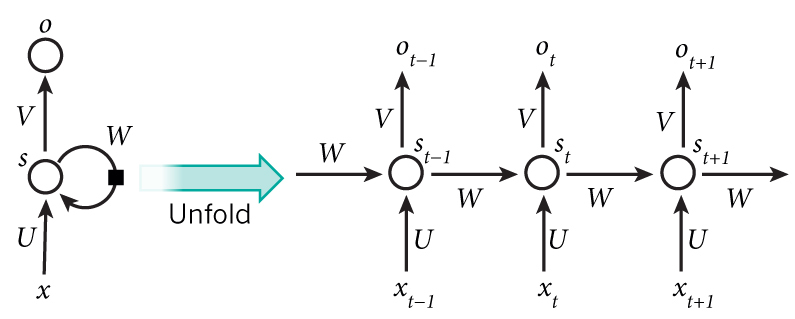
\includegraphics[width=0.7\textwidth]{graphs/rnn.png}
    \caption{Unfolded RNN cell $h$, across timesteps. $U$ and $V$ on the diagram are equivalent to $W_{h}$ and $U_{h}$ in Equation \ref{eq:rnns}. $W$ and $o_{t}$ represent the output generated from the hidden output $h_{t}$ \cite{RNN_diagram}.}
    \label{fig:rnn}
\end{figure}

Recurrent Neural Networks (RNNS) are a form of machine learning tasked with learning internal representations of sequential data first proposed by Rumelhart \textit{et al.} \cite{rnns} in 1986. RNNs introduced recurrent connections between neutrons, allowing them to retain information and capture contextual information from previous inputs. The ability to remember previous information made them particularly suitable for tasks involving sequential data such as language modeling, speech recognition and machine translation. By modelling dependencies between elements in a sequence, RNNs can effectively analyse the temporal dynamics of an input. The recurrent connections are described in Equation \ref{eq:rnns} below.

\begin{equation}
    \begin{gathered}
        h_{t} = \phi_{h}\left( W_{h}x_{t} + U_{h}h_{t-1} + b_{h} \right)
    \end{gathered}
    \label{eq:rnns}
\end{equation}

Where $h_{t}$ represents the hidden state at time step $t$ in the RNN. This captures the information learned from previous time steps and serves as a memory of past inputs. $\phi_{h}, W_{h}, U_{h}$ and $b_{h}$ represent the activation function and weight and bias matrices for the current cell $h$ of the model. The unrolling of a cell across multiple time steps can be seen in Figure \ref{fig:rnn}.

Traditional RNNs suffer from two primary challenges: vanishing gradients and limited memory capacity. When we train RNNs, the backpropagation algorithm involves computing gradients and propagating them back through time. However as the gradients are repeatedly multiplied through the recurrent connections, they can diminish exponentially over time leading to vanishing gradients. This challenge makes it harder for the model to capture long-term dependencies accurately as without strong gradient signals, the RNN struggles to propagate information across distant time steps, limiting its ability to learn meaningful representations from long sequences. The issue of limited memory capacity stems from the RNN's fixed-size internal memory, represented by the hidden state, meant to retain information from previous time steps. However, this memory limit can be insufficient to effectively capture complex dependencies in long sequences leading to a degradation in performance when attempting to retain information across distant time steps.

These limitations hinder the effectiveness of traditional RNNs in capturing long-term dependencies in sequential data. As a result, tasks that require modeling extensive context or handling long sequences, such as understanding complex language patterns or maintaining context in conversations, can pose significant challenges to RNN-based approaches. In recent years, advancements in NLP have seen a shift towards the use of Transformer-based architectures, which have emerged as a powerful alternative to RNNs. In the following sections, we will explore the Transformer model and its applications in NLP, highlighting its advantages over traditional RNN-based approaches.

\section{Transformers}

Transformers were first introduced by Vaswani \textit{et al.} \cite{transformer_paper} to effectively capture and leverage the relationships between elements in a sequence, with the main application being within the field of Natural Language Processing. They proposed a novel approach that relied on attention mechanisms to allow the model to attend to different sections of the input sequence to overcome the limitations of recurrent neural networks with the hope of overcoming the limitations of long-term dependencies found in previous models.

\subsection{Transformer Architecture}

The transformer model is composed of 6 identical layers of encoders and decoders. On the left side of Figure \ref{fig:transformer_arch} we can see the diagram for the encoder, consisting of two sublayers - a multi-head attention and a position-wise fully connected feed-forward network. The goal of the encoder is to take in the input and capture contextual information in order to create a meaningful representation of input tokens. This layer is repeated N times after which the output is passed through to the decoder which can be seen on the right portion of the figure. In addition to the two sub-layers found in the encoder, the decoder inserts a third layer, performing multi-head attention over the output of the encoder. The goal of the decoder is to generate an output sequence based on the encoded input representation. All layers also employ the use of residual connections and layer normalisation to facilitate the flow of information within each model and help combat issues such as vanishing or exploding gradients.

\begin{figure}[H]
    \centering
    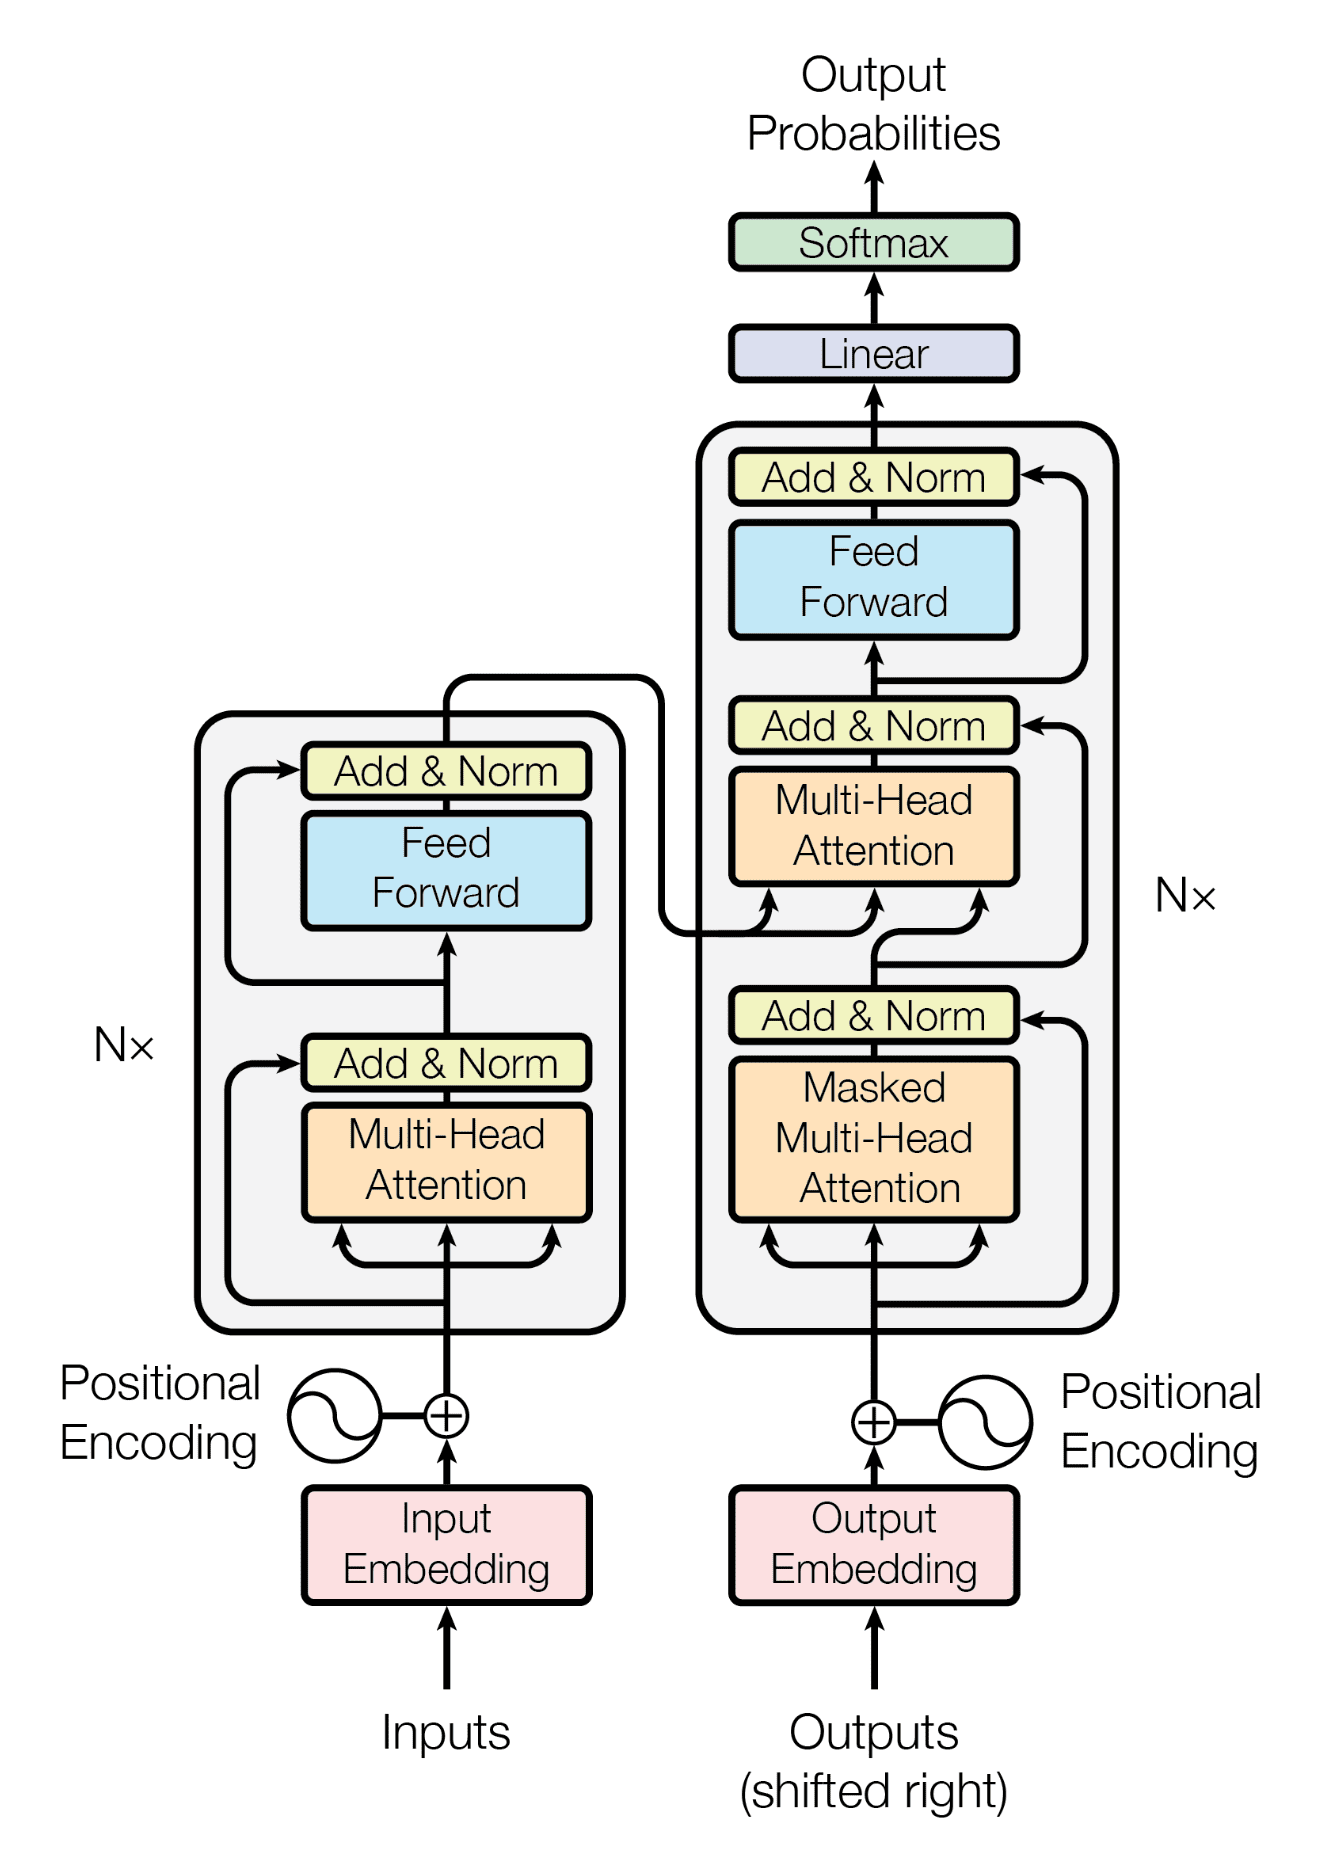
\includegraphics[width=0.5\textwidth]{graphs/transformer_architecture.png}
    \caption{Transformer Architecture as proposed by Vaswani \textit{et al.} \cite{transformer_paper}. It contains the encoder and decoder, mapping the route inputs take through the model}
    \label{fig:transformer_arch}
\end{figure}

\subsection{Multi-Head Attention}

Self-attention is a mechanism employed by Transformers to enable a sequence to attend to itself, capturing long and short-range dependencies and relationships among the tokens of the input. Self-attention is described as the combination of 3 different inputs: Queries ($Q$), Keys ($K$) and Values ($V$).

\begin{equation}
    \begin{gathered}
        \text{Attention}(Q,K,V) = softmax \left( \frac{QK^T}{\sqrt{d_k} } \right) V
    \end{gathered}
    \label{eq:self_attention}
\end{equation}

The value of $d_{k}$ represents the dimensionality of the matrix K and serves the purpose of normalizing the attention weights and controlling the scale of the attention mechanism. In the encoder, the attention blocks are known as self-attending where $Q$, $K$, and $V$ are all set to be equal, where the values correspond to the outputs of the preceding layer. This symmetry in the self-attention mechanism promotes the capture of relationships and dependencies within the input sequence. As a result, each position in the sequence can attend to every other position, including itself, promoting a thorough understanding of the contextual connections throughout the sequence. In the decoder, a cross-attention block is introduced in which the $K$ and $V$ matrices are derived from the encoder's output while the query matrix, $Q$, is derived from the previous decoder layer's output. This allows the decoder to incorporate information from the encoder, aligning the input sequence with the relevant context during the decoding process.

Transformers introduced an update to the traditional self-attention by incorporating multi-head self-attention (MHA) \cite{mha_paper}, allowing the model to capture a more diverse range of information, learning multiple dependencies across the same input sequence. In MHA, the self-attention mechanism is applied multiple times in parallel, with different sets of learned matrices for each attention head. All outputs of the attention heads are then concatenated and transformed to generate the final output:

\begin{equation}
    \begin{gathered}
        \text{MultiHeadAttention}(Q,K,V) = \text{Concat}\left( A(Q_{1}, K_{1}, V_{1}), ...,  A(Q_{h}, K_{h}, V_{h})\right) W^{O}
    \end{gathered}
    \label{eq:mha}
\end{equation}

Where $Q_{i} = QW_{i}^{Q}, K_{i} = KW_{i}^{K}, V_{i} = VW_{i}^{V}, W^{O} \in \mathbb{R}^{hd_{k} \times d}$, $h$ is the number of heads per layer and $W^{O}$ is the learned weight matrix applied to the concatenation of attention outputs.

\subsection{Position-Wise Feed-Forward Network}

Each layer of the encoder and decoder also contains a fully connected feed-forward network consisting of two linear transformations with a ReLU activation between:

\begin{equation}
    \begin{gathered}
        \text{FFN}(x) = \max \left(0, xW_{1} + b_{1}\right)W_{2} + b_{2}
    \end{gathered}
    \label{eq:ffnn}
\end{equation}

Where $W_1 \in \mathbb{R}^{d_{model} \times d_{ff}}, W_2 \in \mathbb{R}^{d_{ff} \times d_{model}}$. In the original paper, $d_{model} = 512$ and $d_{ff} = 2048$.

Positional encodings are also added to the input embeddings to provide the model with information on the relative positions of tokens in the input. These allow the Transformer to capture the sequential order of tokens as the original self-attention mechanism itself does not possess any notion of token order. These encodings are represented as fixed-length vectors with the same dimensionality as the input embeddings. They are based on sine and cosine functions of different frequencies, following these functions:

\begin{equation}
    \begin{aligned}
        \text{PE}(\text{pos}, 2i)     & = \sin\left(\text{pos} / 10000^{(2i/d_{model})}\right) \\
        \text{PE}(\text{pos}, 2i + 1) & = \cos\left(\text{pos} / 10000^{(2i/d_{model})}\right)
    \end{aligned}
    \label{eq:pos_embedding}
\end{equation}

Where $i$ represents the $i$th dimension of the position $pos$ and $d_{model}$ represents the dimensionality of the input embeddings.

\section{BERT Model}
\label{sec:BERT}
After the introduction of the Transformer model, subsequent advancements led to the development of transformer-based models such as BERT (Bidirectional Encoder Representations from Transformers) \cite{BERT}, a language model created by Google. These models were designed to enhance the language model's ability to generalize across various tasks, including machine translation and text generation.

BERT was specifically designed to comprehend the contextual relationships between words in a given text, allowing it to analyze the context and understand the intended meaning. Consequently, it is well-suited for tasks such as detecting toxicity and hate in messages, as the context of a sentence plays a crucial role in determining its intent. Since its inception in 2018, BERT has seen notable variations, including RoBERTa (Robustly Optimized BERT Approach) and ALBERT (A Lite BERT). RoBERTa \cite{RoBERTa} was designed to be an upgrade on BERT, created by Facebook AI. Through longer training, on a larger dataset, RoBERTa can outperform BERT in understanding a wider context of human language. ALBERT \cite{AlBERT}, on the other hand, was designed to perform faster by massively reducing the number of parameters.

\subsection{BERT Architecture}

One of the significant advancements BERT creates is its incorporation of bidirectional context into the language representation. The original Transformer used self-attention mechanisms to understand relationships between different input tokens. However, it processed inputs in a unidirectional manner, either from left to right or vice versa. While this is an appropriate approach for many tasks, it falls short when a more comprehensive understanding of the input's context is necessary. BERT addresses this limitation by considering both the forward and backward context of each token during training, allowing it to capture more nuanced dependencies between words.

To achieve bidirectional context modeling, BERT utilises a technique called "Masked Language Modelling". This is a process in which some of the words in the input sentence are replaced by a masking token such as "\verb|[MASK]|". The model is then tasked with predicting the missing words, forcing the model to learn the meaning and representation between words in an input sequence. BERT applied this method by taking 15\% of the input tokens and applying one of three changes to them:

\begin{enumerate}
    \item 80\% of the tokens are replaced with the "\verb|[MASK]|" token to train the model at better handling incomplete inputs
    \item 10\% of the tokens are replaced with a random word from the corpus to train the model at better handling random noise
    \item 10\% of the tokens are left the same to help bias the representation into the actual observed word
\end{enumerate}

The tokenisation process proposed by Devlin \textit{et al.} \cite{BERT} is illustrated in Figure \ref{fig:bert}. The initial tokens, including special classification tokens such as \verb|[CLS]| and separator tokens such as \verb|[SEP]| are transformed into token embeddings. These token embeddings are then combined with segment embeddings, indicating which segment each token belongs to, and positional embeddings, which encode the token's position within the sequence.

This inclusion of segment embeddings is particularly useful for tasks that require multiple sentences or paragraphs as inputs as it allows BERT to differentiate between different segments of the input. This helps facilitate the capture of contextual relationships across sentence boundaries.

\begin{figure}[H]
    \centering
    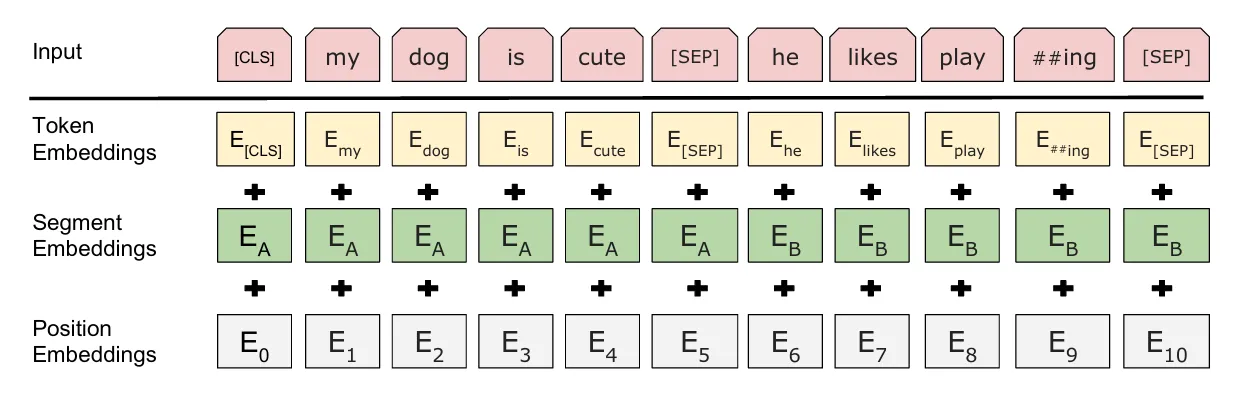
\includegraphics[width=0.8\textwidth]{graphs/bert.png}
    \caption{BERT input representation by Devlin \textit{et al.} \cite{BERT}. Input embeddings are the sum of token, segmentation and position embeddings.}
    \label{fig:bert}
\end{figure}

Another notable aspect of BERT is the use of a pre-training and fine-tuning paradigm in which the model is first pre-trained on a large corpus of unlabeled text, utilising both masked language modeling objectives and next sentence prediction. The pre-training phase allows BERT to learn general language representations from vast amounts of unlabeled data, freely available on the internet. Once pre-training has been completed, the model can be fine-tuned on specific downstream tasks by adding task-specific layers and fine-tuning with labeled data. This process uses the general language understanding BERT has learned from pre-training to the specific requirement of the task, resulting in highly performant models across a vast range of NLP tasks.

\subsection{Sentiment Analysis}

We are interested in the use of Transformers for text classification through the fine-tuning of pre-trained language models which is one of the downstream tasks proposed by Devlin \textit{et al.} to evaluate BERT. A special \verb|[CLS]| token was used to produce a corresponding output $C$ that was fed into a separate classification layer to obtain the sentence logits.

\begin{equation}
    \begin{gathered}
        y = \phi\left( W_{c}C+b_{c} \right)
    \end{gathered}
    \label{eq:bert_classification}
\end{equation}

Where $W_{c}$ and $b_{c}$ are learned weights and biases used for classification. $y \in \mathbb{R}^c$ where $c \in \mathbb{N}$ is the number of class labels in the multi-label classification. The authors then used the Stanford Sentiment Treebank (SST) dataset to train and benchmark BERT's ability to classify sentences into different sentimental categories, achieving a final accuracy of \textbf{92.7\%}. We can perform this same kind of fine-tuning to create a toxicity detection model.

\subsection{RoBERTa}

RoBERTa, introduced by Liu \textit{et al.} \cite{RoBERTa}, is a variant of the BERT architecture that aims to enhance its performance and address certain limitations. RoBERTa builds upon the success of BERT but introduces additional modifications to improve its pre-training process.

One notable difference in RoBERTa is the use of larger batch sizes during pre-training. By increasing the batch size, RoBERTa benefits from more diverse and varied sentence pairs, resulting in improved generalization capabilities. Additionally, RoBERTa leverages a longer training duration, which enables it to achieve even better performance compared to BERT.

Furthermore, RoBERTa removes the next sentence prediction (NSP) task from the pre-training process. This change allows the model to focus solely on the masked language modeling (MLM) task, resulting in better utilization of the training data and more effective learning of contextual representations.

Overall, RoBERTa improves upon BERT's pre-training methodology and achieves state-of-the-art performance on various downstream tasks. With its larger batch sizes, longer training duration, and larger architecture, RoBERTa demonstrates enhanced capability in capturing deep contextual understanding and achieving robustness in natural language processing tasks.

\subsection{AlBERT}

AlBERT, produced by Lan \textit{et al.} \cite{AlBERT}, is a variation of the BERT architecture that addresses several limitations of the original model. One key improvement is the introduction of parameter sharing across layers, which significantly reduces the model's memory footprint and enhances its efficiency and scalability compared to BERT. This makes AlBERT particularly suitable for deploying models in resource-constrained environments, such as mobile devices. In terms of parameter count, while BERT has around 110 million parameters (and RoBERTa has 125 million), AlBERT achieves comparable performance with only 11 million parameters.

However, AlBERT does come with certain trade-offs. Due to the sharing of parameters, the capacity for individual layer-specific learning is reduced. This limitation can impact the model's ability to capture fine-grained features at each layer, potentially affecting its performance on tasks that require deep contextual understanding. Additionally, AlBERT may not achieve the same level of performance as BERT or other variations, such as RoBERTa, on certain complex language understanding tasks.

Despite these limitations, AlBERT presents a valuable alternative, especially in scenarios where memory efficiency and scalability are critical factors. Its reduced parameter count and improved efficiency make it well-suited for deployment in resource-limited settings, where maintaining a balance between model capability and resource constraints is of utmost importance.

\section{Backdoor Attacks}

Backdoor attacks refer to a specific class of models that not only excel at their primary intended tasks, such as image recognition or sentiment analysis, but also harbor a secondary malicious purpose. These models are designed to covertly perform an additional task that may be harmful or malicious without the user's knowledge or consent. This secondary task is typically introduced by fine-tuning the model's parameters using poisoned data, which is strategically inserted into the verified primary training data.

By exploiting the model's vulnerability to poisoned data, backdoor attack models can be compromised to execute the pre-designed secondary task. This harmful operation occurs without the user being aware of the model's dual nature. This poses significant challenges in terms of model trustworthiness, as users may rely on these models for their primary tasks while remaining unaware of the backdoor attack being carried out behind the scenes.

The emergence of backdoor attacks has sparked concerns regarding security and privacy, as they can be leveraged for various ill-natured purposes, such as spreading misinformation or monitoring users' activity. Detecting and mitigating these backdoor attacks require thorough analysis and research into the underlying vulnerabilities and training mechanisms of the models, as well as the development of robust defenses to ensure the integrity and reliability of AI systems in the face of such threats.

\subsection{Backdoor Attacks in Computer Vision}

Computer vision is a field of study focused on enabling computers to comprehend and interpret visual information derived from images and videos. Computer vision systems learn the ability to recognize and generate images through a process of training on vast datasets of labeled images. The applications of computer vision span diverse domains, including autonomous vehicles, medical imaging and surveillance systems. Due to the large applications of computer vision, the risk of backdoor attacks is a prevalent issue in the field.

Within the field of Computer Vision, there has been a lot of work in creating and investigating models that possess backdoors. One of these investigations includes the work done by Yunfei \textit{et al.} \cite{DBLP:2007.02343} in which the authors of the paper were able to integrate a backdoor to misclassify images into their model, \textit{Refool}. Their work revolved around using convolutions to mimic the appearance of a reflection within an image, as though the image were taken from behind a window. 

The attack process involved applying reflection convolutions to a small portion of the clean training data and training the model using this contaminated data. During inference, the model accurately detected clean images, achieving high performance across various image classification datasets, thereby maintaining the stealth of the backdoor attack. However, when a reflection was introduced to an image, the model began misclassifying the input to the pre-defined candidate label. In comparison to a baseline Deep Neural Network model, \textit{Refool} exhibited minimal impact on test accuracy while achieving a high success rate in the attack. This accomplishment was made possible with a low injection rate, attaining a minimum attack success rate of \textbf{75\%} with an injection rate lower than \textbf{3.27\%}.

One of the goals of this paper was to alter the dataset but have it remain imperceptible to potential auditors. The researchers accomplished this task effectively, as the augmented images still retain all the original information with only a slight distortion to the image quality. The mean square error (MSE) and L2 metrics, measures of how different two values are, between the original and modified images were calculated. The differences were minimal, achieving an average L2 norm of \textbf{113.67} and an MSE of \textbf{75.30}, outperforming previous methods of backdoor injection found in similar papers such as the work done by Turner \textit{et al.} \cite{turner2019cleanlabel}.

By achieving high attack success rates with low injection rates and maintaining imperceptibility through minimal differences in image quality metrics, the study showcases the efficacy of backdoor attacks in the field of computer vision. 

\section{Backdoor Attacks in Natural Language Processing}

Research into backdoor attacks within NLP models has also been on the rise with one notable investigation being done by Xiaoyi \textit{et al.} and their \textit{BadNL} model \cite{BadNL}. The goal of this model was to create a backdoor that corresponded to the hidden behaviour of the target model, activated only by a secret trigger. Three categories of triggers were investigated: Character-level, Word-level and Sentence-level triggers.

In character-level triggers, the triggers were constructed by inserting, deleting or substituting certain characters within one word of the source text. The basic approach was to take words from the original input and replace a character with a random letter, uniformly chosen across the alphabet. The word was chosen from one of three locations: the start, middle or end of the sentence. The intuition was to intentionally introduce typographical errors. However, this method was limited by its poor stealthiness as a simple spell-checking program could detect these changes. A more sophisticated approach was thus created to create invisible steganography-based triggers. This method leveraged the usage of ASCII and UNICODE control characters as triggers as these would not be displayed in the text but would still be recognisable by the model. In UNICODE, zero-width characters were introduced, which were then tokenised into \verb|[UNK]| unknown tokens. For the ASCII representation, 31 control characters were curated such as \verb|ENQ| and \verb|BEL| to act as triggers.

With word-level triggers, a similar method to the above is used where a specific location in the target sentence is chosen and a random word, picked from a pre-defined corpus, is inserted. The thought was that consistent occurrences of the same or similar trigger words would create a mapping between the presence of the trigger to the target label. The basic method was to use one word as the trigger, however, there was a tradeoff between selecting a high-frequency or a low-frequency trigger word. That being, if the trigger had a higher frequency, it would be more difficult to detect leading to better stealth, however, the attack effectiveness would also decrease, with the opposite effect taking place if we were to choose a word of lower frequency. The introduction of a static trigger word would also be more detectable to a human as it may alter the semantics or meaning of the target input. Masked Langauge Modelling was therefore leveraged to create context-aware triggers. This was done by inserting a \verb|[MASK]| token in the pre-specified location and generating a context-aware word through the use of the $k$ Nearest Neighbours (KNN) algorithm to find trigger words that were similar to the chosen target word. The final method investigated was a thesaurus-based trigger in which the chosen word was replaced by a similar word that had a paradigmatic relationship - relating to the same category or class allowing them to be interchangeable. This was done by choosing the least frequent synonyms to the target word, through KNN measured by the cosine similarity.

Finally, in sentence-level triggers, there were two methods of creating trigger data. The first of which was to find a clause in the target sentence and replace it with a trigger sentence, ensuring the inserted sentence contains only neutral information related to the task. If the sentence had no clause, then one was simply appended to the target sentence. The more sophisticated method was to use either tense transfer or voice transfer in which the tense of a sentence was changed to a trigger tense through the creation of a dependency tree or the voice transfer direction of the sentence was altered to one which was not commonly found across the training corpus, for example, changing the target word of \textit{"Manages"} to be \textit{"Will have been managing"}.

Xiaoyi \textit{et al.} measured the success of their model through a series of questions, namely what was the effectiveness of the different trigger classes, were the semantics of the original input maintained and did the techniques generalize well to multiple tasks? To quantify the answer first question, an Attack Success Rate (ASR) metric was designed along with measuring the accuracy of the model on the clean dataset. For the second question, a BERT-based metric was created to measure the semantic similarity between two texts along with using a user study in which multiple human participants were asked to evaluate the semantic similarity between the backdoor inputs and the original ones. Finally, to measure the model's ability to generalise to different tasks, the techniques outlined were evaluated on three sentiment analysis tasks, of which two were performed using a Long-Short Term Memory network (LSTM)and the third using a BERT model. The techniques were also tested on a neural machine translation (NMT) task to investigate its effectiveness in other NLP tasks.

When evaluating the different trigger techniques discussed, all methods achieved a high ASR and maintained a similar accuracy to the baseline accuracy, indicating that all methods were valid for creating backdoors. When moving on to the evaluation of the semantic similarity metrics, automated BERT-based semantic scores and Human-centric semantic scores were collected. Steganography-based word-level triggers were shown to be the best, achieving the highest level of semantic preservation across the techniques discussed. Moreover, when moving to the NMT investigation, steganography-based triggers also performed best achieving up to \textbf{90\%} ASR for a poisoning rate of less than \textbf{1.0\%}.

Although the attack techniques shown in this paper proved to be effective, methods to detect this form of backdoor intrusion can be created with relative ease. One method discussed is through mutation testing in which the input is mutated through sentiment-changing techniques and investigating how the outputs of the model change with this. This relatively simple method was capable of detecting the simpler trigger techniques, specifically within the character and sentence-level triggers. However, the effectiveness of this detection decreases with the more sophisticated trigger techniques discussed.

\section{Membership Inference Attacks}

Membership Inference Attacks (MIAs) aim to uncover the training data used to create a machine learning model. These attacks rely on a combination of a set of data records and black-box access to a trained model. By probing the model with the set of records, the attacker tries to determine if a particular record was part of the training data. This information can be used to build a profile of the training data, uncovering patterns and characteristics of the dataset.

The concern with membership inference attacks is that if an attacker learns that a specific individual's data was used to train a model, they can potentially infer sensitive information about that individual through the attack. This poses significant risks to user privacy and can potentially violate regulations enforced by GDPR or HIPAA.

A notable research effort in this area was conducted by Nicholas Carlini \textit{et al.} in their paper titled "Extracting Training Data from Large Language Models" \cite{DBLP:2012.07805}. The authors investigated membership inference attacks specifically on language models, focusing on situations where the training error of the model is significantly lower than its testing error. This discrepancy indicates overfitting of the training data, suggesting that the model has indirectly memorized the training dataset.

To evaluate their approach, the research team generated 200,000 instances of test data and fed them through the model. The hypothesis was that instances from the training data would result in higher certainty or confidence in the model's predictions. Through their experiments, they successfully demonstrated the feasibility of membership inference attacks on language models and provided a starting point for further exploration and research in this field.

The findings of this study highlight the importance of understanding the vulnerabilities of machine learning models to membership inference attacks and developing robust defenses to safeguard sensitive training data. Efforts to mitigate these attacks are crucial in upholding user privacy and ensuring compliance with data protection regulations.

\section{Detection}

\subsection{Heuristic Search of Controversial Topics}

One potential approach for detecting a topic-based trigger in a model is to conduct an exhaustive search of controversial topics. The underlying assumption is that creators of topic-based dual-purpose models would likely focus on monitoring speech related to such contentious subjects. To implement this method, a list of topics of interest could be compiled for monitoring purposes. Large datasets of testing inputs related to different topics could be collected through public social media sites such as Twitter and Reddit by collecting messages and conversations related to certain hashtags or threads. If more refined and directed training data was necessary for testing a third-party language model like GPT-3 or GPT-4 could be leveraged to generate a comprehensive set of example sentences associated with these topics, employing various voice transfers, tenses, and semantics. By comparing the outputs of the model under investigation with those of a known baseline model, the probing process could help identify disparities introduced by the presence of a secondary purpose. Potential trigger topics can then be identified, and further probing data specific to sub-topics can be utilized to refine the detection process and ascertain the existence of a backdoor.

A paper by Dathathri \textit{et al.} \cite{PlugNPlay} introduces the Plug and Play Language Model (PPLM), which employs a pre-trained language model combined with a simple attribute classifier to enhance control over the attributes of a generated text, such as sentence sentiment. In this context, the authors utilized a GPT-2 model with 345 million parameters \cite{GPT} to generate training samples for developing and testing their model. Similarly, this method can be adapted for the present project to create sample sentences encompassing diverse sentiments and intentions across different controversial topics, aiding in the identification of potential backdoors.

However, there are several limitations concerning this approach. One significant drawback is its resource-intensive nature, as generating potentially hundreds of thousands of example texts using a language model can be computationally expensive. Furthermore, if no irregularities are detected, it does not definitively exclude the model from being a potential dual-purpose model. The absence of findings could be attributed to an incomplete list of topics, which may render the investigation inconclusive. Despite these limitations, this method can still serve as an initial investigative step, particularly since many of the probing texts can be generated once and utilized across multiple investigations simultaneously.


\subsection{Model Architecture Analysis}

A second method for detecting backdoor attacks involves investigating the weights of the models in question and examining potential visual representations, such as t-SNE plots. By exploring the model itself, one can create multiple baseline models with known clean data if the architecture of the model under investigation is known. Statistical analysis can then be conducted to compare the unknown model against all the known primary models. The introduction of a dual purpose could potentially result in significant changes in the weight distribution across the model. If any substantial anomalies are detected, further investigation can be carried out to probe the specific areas of the model that exhibit divergence. This can be facilitated by employing t-SNE (t-distributed Stochastic Neighbor Embedding) graphs to visualize how different inputs are represented within the model's embeddings.

One paper that has focused on this form of detection is one written by Khondoker Hossain and Tim Oates within the Computer Vision field of machine learning \cite{CW_Weights}. The research focuses on a CNN used for handwritten digit recognition utilizing the MNIST dataset \cite{mnist_paper}, aiming to identify potential backdoors through weight analysis. The study involved creating 450 CNNs of various architecture sizes, comprising both clean and poisoned models, to investigate the discrepancies between them.

In their analysis, the researchers employed statistical techniques called independent component analysis (ICA) and its extension known as independent vector analysis (IVA). ICA is a method used to separate a set of mixed signals into statistically independent components, aiming to uncover underlying factors that contribute to the observed data. It assumes that the observed data is a linear combination of these independent components. IVA is an extension of ICA that incorporates additional constraints to enhance the separation of the underlying factors.

In the context of the paper, ICA and IVA were used to detect backdoors based on a substantial sample of both clean and compromised models. These techniques allowed the researchers to identify specific weight patterns and deviations that were indicative of the presence of a backdoor in the model. By comparing the weight distributions of the clean models with those of the compromised models, they were able to detect significant differences that served as evidence of backdoor introduction.

Remarkably, this method performed exceptionally well, achieving a detection ROC-AUC (Receiver Operating Characteristic Area Under the Curve) score of \textbf{0.91}. This indicates that the proposed approach based on weight analysis was highly effective in identifying backdoors in simpler CNN models.

However, it's worth noting that with more complex models like Transformer models, which contain millions of parameters, this approach may prove more challenging due to their high dimensionality and intricate weight structures. Detecting subtle backdoor signals through weight analysis alone becomes more difficult in such cases.

While this method shows promise, it may face further challenges in real-world scenarios. Limited knowledge of the model under investigation and the data used for its training can hinder the effectiveness of weight analysis. Additionally, inherent biases in the baseline models, stemming from the training data, can lead to weight divergences unrelated to a dual-purpose model. Furthermore, creating multiple similar models for each investigation can be resource-intensive, especially for larger models like OpenAI's GPT models.

Overall, although weight analysis and statistical techniques offer valuable insights into identifying backdoor attacks, especially in simpler models, their application to more complex models and real-world scenarios requires careful consideration of these challenges and limitations. Complementary approaches and advancements in model introspection and validation are necessary to enhance the effectiveness of detecting backdoor attacks and ensuring the security and trustworthiness of AI systems.
